\section{简介}
使用 SimplePaper 很简单,创建一个 tex 文件,在其中输入以下内容。就可以编译出一个简单的 PDF 文件了,如\cref{{fig:pdf_example}}所示。如果需要写英文论文,只要将 cn 改成 en 即可。

\begin{lstlisting}
\documentclass[cn]{simplepaper}
\begin{document}
    \title{SimplePaper 模版使用说明}
    \author{朱亮亮}
    \date{\today}
    \maketitle
    这是一个模版使用说明。

    正文...
\end{document}
\end{lstlisting}
\begin{figure}[htb!]
    \centering
    \fbox{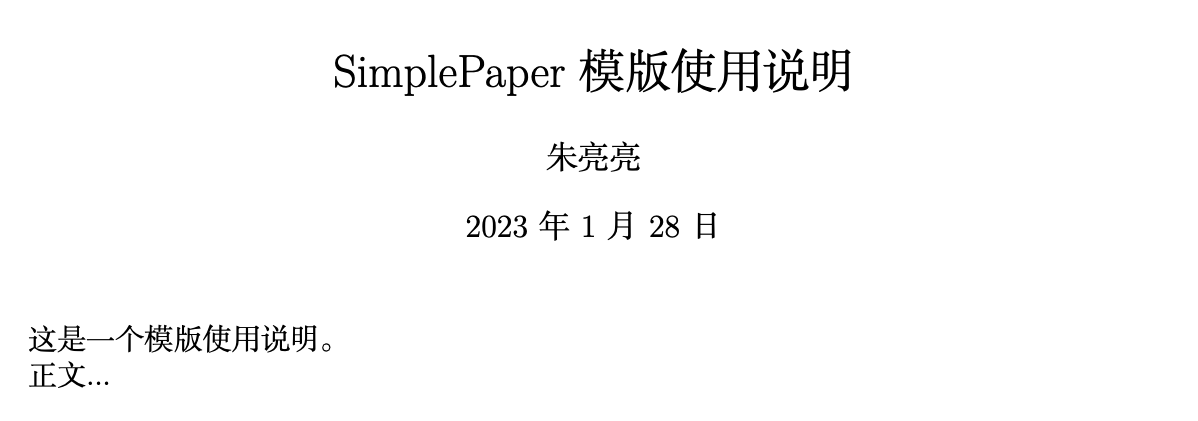
\includegraphics[width=.8\textwidth]{./img/pdf_example.png}}
    \caption{编译结果}
    \label{fig:pdf_example}
\end{figure}
此外,SimplePaper 提供中文字体选择。比如,下面的代码就使用了方正字体:
\begin{lstlisting}
\documentclass[cn, founder]{simplepaper}
\end{lstlisting}

在一般情况下,如果论文中存在大量的图片,那么编译的过程中编译器往往会对图片进行压缩,从而减少最后输出的 PDF 文件的大小。但是,这样做增加编译时间,而在论文写作过程中难免会反复修改,为了减少等待时间,SimplePaper 提供了 nocomp 选项,用于禁用图片压缩。此时的编译时间会大大减少,但是 PDF 文件大小会大大增加,只建议在写作时使用。

论文初稿完成后,往往需要发给导师和同学们修改修改,这时候就需要将论文模版设置为 preprint 模式,这样编译的过程中图片就会被压缩(但不影响显示效果),从而减少 PDF 文件的大小。与此同时,论文页面的左侧空白出会有行号(nocomp 模式也有),方便在线交流时指出问题的具体位置。当论文修改完成后,可以将模版设置为 final 模式,此时会开启图片压缩,并且最终的 PDF 文件不再有行号。具体使用方法和字体选项相同,比如下面的代码就使用了 nocomp 模式。
\begin{lstlisting}
\documentclass[cn, nocomp]{simplepaper}
\end{lstlisting}


总的来说,SimplePaper 模版提供了三个选项,分别是语言选择、字体选择、字体大小选择和样式选择:

\paragraph{语言 lang}
\begin{itemize}
    \item en (默认选项,使用英文模版,推荐使用PdfLaTeX编译器)
    \item cn (使用中文模版,推荐使用XeLaTeX编译器)
\end{itemize}

\paragraph{字体 font}
\begin{itemize}
    \item ctexfont (默认选项,使用 ctex 默认配置的中文字体)
    \item founder (方正字体,更好看,需要自行安装对应字体)
    \item nofont (不设置中文字体,需自行指定)
\end{itemize}

\paragraph{字体大小 fontsize}
\begin{itemize}
    \item 10pt 
    \item 11pt (默认)
    \item 12pt 
\end{itemize}

\paragraph{样式 style}
\begin{itemize}
    \item nocomp (默认选项,不压缩图片,编译速度快,PDF文件大,左侧有行号)
    \item preprint (压缩图片,编译速度慢,PDF文件小,左侧有行号)
    \item final (压缩图片,编译速度慢,PDF文件小,左侧无行号)
\end{itemize}